\let\negmedspace\undefined
\let\negthickspace\undefined
\documentclass[journal]{IEEEtran}
\usepackage[a5paper, margin=10mm, onecolumn]{geometry}
%\usepackage{lmodern} % Ensure lmodern is loaded for pdflatex
\usepackage{tfrupee} % Include tfrupee package

\setlength{\headheight}{1cm} % Set the height of the header box
\setlength{\headsep}{0mm}     % Set the distance between the header box and the top of the text

\usepackage{gvv-book}
\usepackage{gvv}
\usepackage{cite}
\usepackage{amsmath,amssymb,amsfonts,amsthm}
\usepackage{algorithmic}
\usepackage{graphicx}
\usepackage{textcomp}
\usepackage{xcolor}
\usepackage{txfonts}
\usepackage{listings}
\usepackage{enumitem}
\usepackage{mathtools}
\usepackage{gensymb}
\usepackage{comment}
\usepackage[breaklinks=true]{hyperref}
\usepackage{tkz-euclide} 
\usepackage{listings}
% \usepackage{gvv}                                        
\def\inputGnumericTable{}                                 
\usepackage[latin1]{inputenc}                                
\usepackage{color}                                            
\usepackage{array}                                            
\usepackage{longtable}                                       
\usepackage{calc}                                             
\usepackage{multirow}                                         
\usepackage{hhline}                                           
\usepackage{ifthen}                                           
\usepackage{lscape}
\usepackage{multicol}
\begin{document}

\bibliographystyle{IEEEtran}
\vspace{3cm}

\title{12.442}
\author{EE25BTECH11012-BEERAM MADHURI}
% \maketitle
% \newpage
% \bigskip
{\let\newpage\relax\maketitle}

\renewcommand{\thefigure}{\theenumi}
\renewcommand{\thetable}{\theenumi}
\setlength{\intextsep}{10pt} % Space between text and floats


\numberwithin{equation}{enumi}
\numberwithin{figure}{enumi}
\renewcommand{\thetable}{\theenumi}


\textbf{Question}:\\
 Eigen values of the matrix
$\begin{pmatrix}5 & 3 \\1 & 4\end{pmatrix}$
are

\begin{enumerate}
\begin{multicols}{4}
\item [a)] $-6.3$ and $-2.7$
\item [b)] $-2.3$ and $-6.7$
\item [c)] $6.3$ and $2.7$
\item [d)] $2.3$ and $6.7$
\end{multicols}
\end{enumerate}

\textbf{Solution:}\\
Let 
\begin{align}
A = \begin{bmatrix} 5 & 3 \\ 1 & 4 \end{bmatrix}\\
A = \lambda I
\end{align}
where `$\lambda$' are eigen values.
\begin{align}
\begin{vmatrix} A - \lambda I \end{vmatrix} = 0
\end{align}
\begin{align}
\begin{vmatrix} \begin{bmatrix} 5 & 3 \\ 1 & 4 \end{bmatrix} - \lambda \begin{bmatrix} 1 & 0 \\ 0 & 1 \end{bmatrix} \end{vmatrix} = 0
\end{align}
\begin{align}
\begin{vmatrix} \begin{bmatrix} 5-\lambda & 3 \\ 1 & 4-\lambda \end{bmatrix} \end{vmatrix} = 0
\end{align}
\begin{align}
(5-\lambda)(4-\lambda) - 3 = 0\\
20 - 9\lambda + \lambda^2 - 3 = 0\\
\lambda^2 - 9\lambda + 17 = 0\\
\lambda_1 = 6.3\\
\lambda_2 = 2.7
\end{align}
Hence eigen values of given matrix are 2.7 and 6.3.\\
$\therefore$ Option C is correct.

\begin{figure}
    \centering
    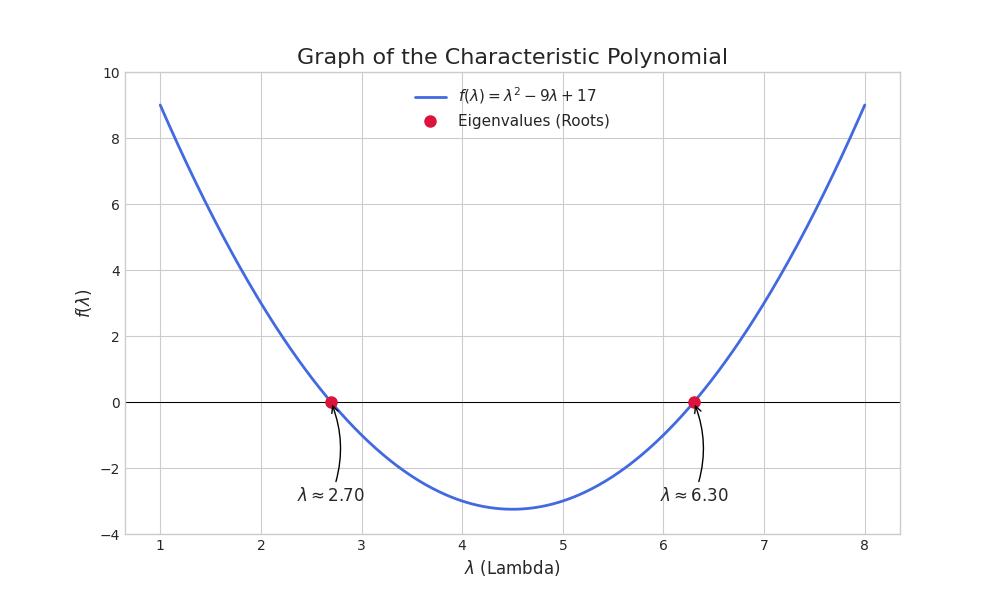
\includegraphics[width=0.85\columnwidth]{figs/graph23.png}
    \caption{12.442}
    \label{fig:placeholder}
\end{figure}
\end{document}
